\section{Bayesian inference for the Gaussian distribution}

\subsection{The univariate Gaussian}
\begin{align}
t &\sim \mathcal{N}(\mu,\sigma^2)\\
p(t|\mu, \sigma^2)&=\frac{1}{\sqrt{2\pi\sigma^2}}\exp\left( -\frac{1}{2}\left(\frac{t-\mu}{\sigma} \right)^2\right)
\end{align}
\begin{itemize}
\item 
The Gaussian has \emph{mean} $\mu$ and \emph{variance} $\sigma^2$ and \emph{precision} $\beta=1/\sigma^2$
\end{itemize}

\begin{bbbox}{The univariate Gaussian}

\begin{flalign*}
	\mu = 0; \sigma^2 = 1, \\
	P(t) = \frac{1}{\sqrt{2\pi}} \mbox{e}^{-\frac{1}{2}t^2} \\
	\int_{-\infty}^{\infty} P(t) 
		&= \frac{1}{\sqrt{2\pi}} \int_{-\infty}^{\infty} \mbox{e}^{-\frac{1}{2}t^2} dt\\
		&= \frac{1}{\sqrt{2\pi}} \sqrt{2\pi} = 1
\end{flalign*}

\begin{itemize}
\item  Q: What are the \emph{mode} and the \emph{median} of the Gaussian?\\
		  Mode and median of the Gaussian are equal to the mean. This can easily be seen graphically.	
		  
\end{itemize}
\end{bbbox}

\begin{bbbox}{Maximum Likelihood estimation of $\mu$ and $\beta$}

	  \begin{align*}
	  	D &= \{ t_1 , t_2 ,\cdots , t_n \} \\
	  	L(D|\mu,\beta) &= \prod_{n=1}^N \mathcal{N} \left( t_n,\mu,\sigma^2 \right) \\
	  				   &= \sqrt{\frac{\beta}{2\pi}}^N \mbox{e}^{-\frac{\beta}{2} \sum_{n=1}^N \left(t_n - \mu\right)^2} \\
		\log L &= \frac{N}{2} \log \left( \frac{\beta}{2\pi} \right) - \frac{\beta}{2} \sum_{n=1}^N \left(t_n - \mu\right)^2 \\
		\end{align*}
		
		\text{Maximum likelihood solution for the mean } $\mu$ \\
		\begin{align*}
		0 &= \frac{\partial \log L}{\partial \mu} = -\frac{\beta}{2} \sum_{n=1}^N 2 \left(t_n - \mu \right) (-1) \\
		0 &= \sum_{n=1}^N t_n - \sum_{n=1}^N \mu \\
		\mu &= \frac{1}{N} \sum_{n=1}^N t_n \\
		\end{align*}
		
		\text{Maximum likelihood solution for the variance } $\sigma^2 = \frac{1}{\beta}$ \\
		\begin{align*}
		0 &= \frac{\partial \log L}{\partial \beta} = \frac{N}{2\beta} - \frac{1}{2} \sum_{n=1}^N 2 \left(t_n - \mu \right)^2 \\
		\sigma^2 &= \frac{1}{\beta} = \frac{1}{N} \sum_{n=1}^N 2 \left(t_n - \hat{\mu} \right)^2 \\
	  \end{align*}
Q: How would you find the conjugate prior for the Gaussian? \\

\end{bbbox}

\textbf{(very important) aside: Products of Gaussian pdfs are (unnormalized) Gaussians pdfs}
\begin{itemize}
\item Suppose $p_1(x)=\mathcal{N}(x,\mu_1, \frac{1}{\beta_1})$ and $ p_2(x)=\mathcal{N}(x,\mu_2, \frac{1}{\beta_2})$, then  
 \begin{align}
p_1(x) p_2(x) &\propto \mathcal{N}(x, \mu, 1/\beta)\\
\beta&=\beta_1+\beta_2\\
\mu&=\frac{1}{\beta}(\beta_1 \mu_1 +  \beta_2 \mu_2)
\end{align}

\begin{bbbox}{Products of Gaussians}
	Quadratic form for the Gaussian:
	\begin{align*}
		p(t|\mu, \sigma^2) 
		&=\frac{1}{\sqrt{2\pi\sigma^2}}\exp\left( -\frac{1}{2}\left(\frac{t-\mu}{\sigma} \right)^2\right) \\
		&= \frac{1}{Z} \exp \left( \underbrace{a}_{-\frac{1}{2}\text{precision}}x^2 + \underbrace{b}_{\text{precision} \times \text{mean}}x \right) \\
	\end{align*}
	
	We show that the product of two Gaussians $p_1(x)$ and $p_2(x)$ is again Gaussian: \\
	\begin{align*}
	p_1(x) &= \frac{1}{Z_1} \exp \left( -\frac{\beta_1}{2} \left(x-\mu_1 \right)^2 \right) 	\\
	p_2(x) &= \frac{1}{Z_2} \exp \left( -\frac{\beta_2}{2} \left(x-\mu_2 \right)^2 \right) 	\\
	p_1(x) p_2(x) &= \frac{1}{Z_s} \exp \left( -\frac{\beta_1}{2} \left( x - \mu_1 \right)^2
					  -\frac{\beta_2}{2} \left( x - \mu_2 \right)^2	\right)\\
				  &= \frac{1}{Z_q} \exp \left( -\left( \frac{\beta_1}{2} + \frac{\beta_2}{2}\right) x^2
	                 + 2\left( \frac{\beta_1}{2} \mu_1 + \frac{\beta_2}{2} \mu_2 \right) x \right)\\
	\beta &= \beta_1 + \beta_2 \\
	\beta \mu &= = \beta_1 \mu_1 + \beta_2 \mu_2 \\
	\mu &= \frac{1}{\beta} \left( \beta_1 \mu_1 + \beta_2 \mu_2 \right)
	\end{align*}
	The quadratic form helps us to simply read out the parameters of our resulting Gaussian. We will see later that this observation comes in handy for Bayesian inference with Gaussians.
\end{bbbox}
 
In general:
\begin{align}
p_1(x) p_2(x) ... p_n(x) &\propto \mathcal{N}(x, \mu, 1/\beta)\\
\beta&=\sum_n \beta_n\\
\mu&=\frac{1}{\beta} \sum_n \mu_n \beta_n
\end{align}

 
This is also true for multivariate Gaussians!

\end{itemize}



\subsection{Bayesian inference for Gaussians}

\begin{itemize}
\item Suppose we are given data $D=\{x_1, \ldots, x_N\}$. 
\item We assume that the data is Gaussian-distribution with known variance $\sigma^2$ and unknown mean $\mu$.
\item Our prior for $\mu$ is Gaussian: $\mu \sim \mathcal{N}(\mu_o, \sigma^2_o)$
\item Posterior distribution over $\mu$ given the data: [on board] 
\end{itemize}

\begin{bbbox}{Posterior inference for the Gaussian}
	Here we want to derive the posterior  distribution for the mean of a Gaussian. For now we will assume that the variance $\sigma^2$ of our Gaussian is known and that the only parameter of interest is $\mu$. \\
	We define a prior over $\mu$:   $p(\mu) = \mathcal{N}(\mu_0, \sigma^2_0)$ which is again Gaussian. \\
	From before we know that our posterior distribution over $\mu$ is again Gaussian:
	\begin{align*}
		p(\mu|\sigma^2, \underbrace{\mu_0, \sigma_0^2}_{Prior},D)	
		            &\propto p(D|\mu,\sigma^2,\mu_0, \sigma_0^2) p(\mu|\mu_0, \sigma_0^2) \\
		            &\propto \prod_{n=1}^N \mathcal{N}(x_n,\mu,\sigma^2) \mathcal{N}(\mu,\mu_0, \sigma_0^2) \\
		            &\propto \mathcal{N}(\mu,\mu_{post},\sigma_{post}^2) \\
		\frac{1}{\sigma_{post}^2} &= \sum_{n=1}^N \left(\frac{1}{\sigma^2} \right) + \frac{1}{\sigma_0^2} \\
		\sigma_{post}^2 &= \frac{1}{\frac{N}{\sigma^2} + \frac{1}{\sigma_0^2}} \\
		\mu_{post} &= \sigma_{post}^2 \left( \sum_{n=1}^N \left( x_n\frac{1}{\sigma^2} \right) + \mu_0 \frac{1}{\sigma_0^2} \right)
	\end{align*}
	
Behaviour for large $N$: [on board]
\begin{align*}
	\text{for large N: } \sigma_{post}^2 = \frac{\sigma^2}{N} \\
	\mu_{ML} &= \frac{1}{N} \sum_{n=1}^N x_n \\
	\mu_{post} &= \frac{\left( \sum_{n=1}^N \left( x_n\frac{1}{\sigma^2} \right) + \mu_0 \frac{1}{\sigma_0^2} \right)}{\frac{N}{\sigma^2} + \frac{1}{\sigma_0^2}} \\
	N \rightarrow \infty: &\mu_{post} = \mu_{ML} \\
	\sigma_0^2 \rightarrow 0: &\mu_{post} = \mu_{ML} \\
\end{align*}

\end{bbbox}

\begin{figure}
	\centering
	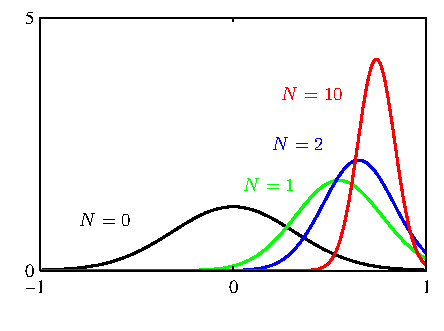
\includegraphics[width=.5\textwidth]{./lecture4/Figure212.pdf}
	\caption{Bishop Figure 2.12}
\end{figure}

\subsubsection{What if the variance is not given?}
\begin{itemize}
\item For simplicity, assume mean to be known.
\item More convenient to work with precision $\lambda=1/\sigma^2$.
\item Conjugate prior: Gamma distribution $\mbox{Gam}(\lambda|a,b)$
\begin{align}
p(\lambda|a, b)=\frac{1}{\Gamma(a)}b^a \lambda^{a-1} exp(-b\lambda)
\end{align}
\item Posterior is $\mbox{Gam}(\lambda|a_N,b_B)$
\begin{align}
a_N &= a + \frac{N}{2}\\
b_N &= b + \frac{1}{2} \sum_{n=1}^N (x_n -\mu)^2
\end{align}

\begin{figure}
\centering
\begin{subfigure}[b]{0.45\textwidth}
                \centering
                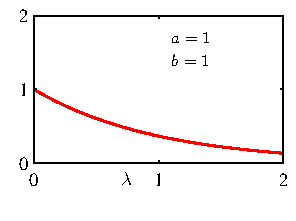
\includegraphics[width=\textwidth]{./lecture4/Figure213b.pdf}
    \end{subfigure}%
	~
	\begin{subfigure}[b]{0.45\textwidth}
                \centering
                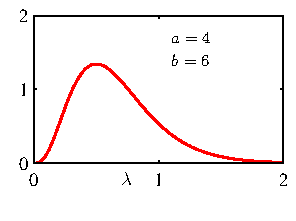
\includegraphics[width=\textwidth]{./lecture4/Figure213c.pdf}
    \end{subfigure}%
   	\caption{Gamma distribution with different parameterizations. The Gamma distribution is a conjugate prior for the presision of a Gaussian. Figures taken from Bishop page 100.}
	
\end{figure}
\end{itemize}


\subsubsection{What if both the mean and the variance are unknown?}
\begin{figure}[h]
	\centering
		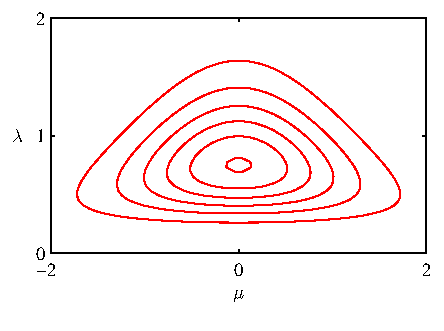
\includegraphics[width=0.7\textwidth]{./lecture4/Figure214.pdf}
		\caption{The Gaussian-Gamma distribution, a conjugate prior for mean and precision of a Gaussian. Bishop figure 2.14, page 102.}
\end{figure}    
\begin{itemize}
\item Conjugate prior: Gaussian-Gamma distribution
\begin{align}
p(\mu,\lambda) & = \mathcal{N}\left(\mu |\mu_o (\beta\lambda)^{-1}\right) \mbox{Gam}(\lambda|a,b)
\end{align}
\end{itemize}
